\documentclass[a4paper,12pt]{article}
\usepackage[margin=0.8in]{geometry}
\usepackage{graphicx}
\usepackage{xcolor}
\usepackage{multicol}
\usepackage{fancyhdr}
\usepackage{amsmath}
\usepackage{wrapfig}
\usepackage{titlesec}
\usepackage{parskip}
\setlength{\parindent}{0pt}
\definecolor{ncertblue}{RGB}{0,153,204}

% Header and Footer
\pagestyle{fancy}
\fancyhf{}
\lhead{\textcolor{ncertblue}{\textbf{82}}}
\rhead{\textcolor{ncertblue}{\textsc{Mathematics}}}
\cfoot{\textcolor{black}{\small Reprint 2025-26}}
\renewcommand{\headrulewidth}{0.5pt}
\renewcommand{\headrule}{\hbox to\headwidth{\color{ncertblue}\leaders\hrule height \headrulewidth\hfill}}

% Section style
\titleformat{\section}{\color{ncertblue}\bfseries}{\thesection}{1em}{}
\setlength{\parindent}{0pt}
\setlength{\parskip}{4pt}

\begin{document}
\pagestyle{fancy}
\fancyhf{}
\lhead{\textcolor{ncertblue}{\textbf{82}}}
\rhead{\textcolor{ncertblue}{\textsc{Mathematics}}}
{\color{ncertblue}\textbf{Theorem 6.2 :} 
\textit{If a line divides any two sides of a triangle in the same ratio, then the line is parallel to the third side.}}

This theorem can be proved by taking a line DE such that 
\[
\frac{AD}{DB} = \frac{AE}{EC}
\]
and assuming that DE is not parallel to BC (see Fig. 6.12). 

If DE is not parallel to BC, draw a line DE$'$ parallel to BC.

\begin{multicols}{2}
So, 
\[
\frac{AD}{DB} = \frac{AE'}{E'C} \quad \text{(Why ?)}
\]
Therefore,
\[
\frac{AE}{EC} = \frac{AE'}{E'C} \quad \text{(Why ?)}
\]

Adding 1 to both sides of above, you can see that E and E$'$ must coincide. (Why ?)

\columnbreak

\begin{center}
    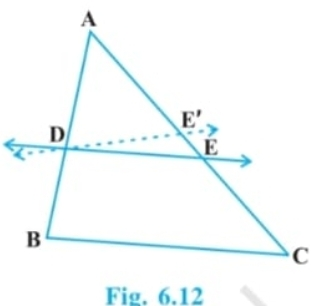
\includegraphics[width=0.9\linewidth]{fig612.jpg}\\
\end{center}
\end{multicols}

Let us take some examples to illustrate the use of the above theorems.

{\color{ncertblue}\textbf{Example 1 :}} If a line intersects sides AB and AC of a $\triangle$ABC at D and E respectively and is parallel to BC, prove that 
\[
\frac{AD}{AB} = \frac{AE}{AC} \quad \text{(see Fig. 6.13).}
\]

{\color{ncertblue}\textbf{Solution :}} DE $\parallel$ BC \hfill (Given)

So,
\[
\frac{AD}{DB} = \frac{AE}{EC} \hfill \text{(Theorem 6.1)}
\]
or,
\[
\frac{DB}{AD} = \frac{EC}{AE}
\]
or,
\[
\frac{DB}{AD} + 1 = \frac{EC}{AE} + 1
\]
or,
\[
\frac{AB}{AD} = \frac{AC}{AE}
\]
So,
\[
\frac{AD}{AB} = \frac{AE}{AC}
\]
\vspace{-20em}
\begin{flushright}
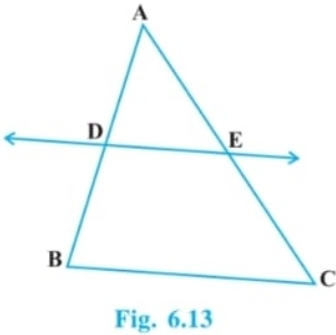
\includegraphics[width=0.38\textwidth]{fig613.jpg}
\end{flushright}
\newpage
% Header and Footer
\pagestyle{fancy}
\fancyhf{}
\lhead{\textcolor{ncertblue}{\textbf{Triangles}}}
\rhead{\textcolor{ncertblue}{\textbf{83}}}
\renewcommand{\headrulewidth}{0.4pt}
\renewcommand{\headrule}{\hbox to\headwidth{\color{ncertblue}\leaders\hrule height \headrulewidth\hfill}}
\fancyfoot[C]{\textcolor{black}{\small Reprint 2025-26}}

% Section title formatting
\titleformat{\section}{\color{ncertblue}\large\bfseries}{}{0em}{}
\titleformat{\subsection}{\color{ncertblue}\bfseries}{}{0em}[]

\textcolor{ncertblue}{\textbf{Example 2 :}} ABCD is a trapezium with AB $\parallel$ DC. E and F are points on non-parallel sides AD and BC respectively such that EF is parallel to AB (see Fig. 6.14). Show that
\[
\frac{AE}{ED} = \frac{BF}{FC}.
\]

\begin{minipage}{0.5\textwidth}
\textcolor{ncertblue}{\textbf{Solution :}} Let us join AC to intersect EF at G (see Fig. 6.15).\\

AB $\parallel$ DC and EF $\parallel$ AB \hfill (Given)

So, EF $\parallel$ DC \hfill (Lines parallel to the same line are parallel to each other)

Now, in $\triangle ADC$,\\
EG $\parallel$ DC \hfill (As EF $\parallel$ DC)\\

So, \[
\frac{AE}{ED} = \frac{AG}{GC} \tag{1}
\] \hfill (Theorem 6.1)

Similarly, from $\triangle CAB$,
\[
\frac{CG}{AG} = \frac{CF}{BF}
\Rightarrow \frac{AG}{GC} = \frac{BF}{FC}
\]

Therefore, from (1) and (2),
\[
\frac{AE}{ED} = \frac{BF}{FC}
\]
\end{minipage}
\hfill
\begin{minipage}{0.45\textwidth}
\centering
\vspace{-5em}
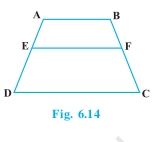
\includegraphics[width=\linewidth]{fig614.jpg}\\
\vspace{-5em}
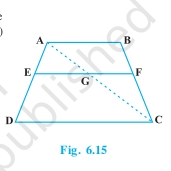
\includegraphics[width=\linewidth]{fig615.jpg}\\
\end{minipage}
\noindent
\begin{minipage}[t]{0.63\textwidth}
\vspace{-10em}\textcolor{ncertblue}{\textbf{Example 3 :}} In Fig. 6.16, $\dfrac{PS}{SQ} = \dfrac{PT}{TR}$ and $\angle PST = \angle PRQ$. Prove that $\triangle PQR$ is an isosceles triangle.


\textcolor{ncertblue}{\textbf{Solution :}} It is given that
\[
\frac{PS}{SQ} = \frac{PT}{TR}
\]

So, ST $\parallel$ QR \hfill (Theorem 6.2)

Therefore, $\angle PST = \angle PQR$ \hfill (Corresponding angles)

Now,
\[
\angle PST = \angle PRQ \Rightarrow \angle PRQ = \angle PQR \Rightarrow PQ = PR
\]

i.e., $\triangle PQR$ is an isosceles triangle.
\end{minipage}
\hfill
\begin{minipage}[t]{0.34\textwidth}
\centering
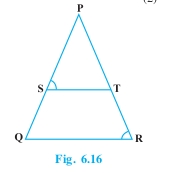
\includegraphics[width=\linewidth]{fig616.jpg}\\[-0.5em]
\end{minipage}

\end{document}
